\chapter{Nearest Centroid Classifier}
\label{ch:ncc}
The first classification algorithm we will look into is the Nearest Centroid Classidfier.
It is a widely used algorithm for classification and is also one of the simplest ones to implement.
We will start by looking at the mathematical background of the algorithm and then implement it in Python.
This will help us to understand how to derive a classification algorithm from a mathematical model as well as the
limitations of machine learning models regarding assumptions it has towards the data.
Apart from this, the NNC is easy to interpret and easy to implement, which is a great starting point to get familiar with 
the Python programming language and the libraries we will use in this book.

\section{Motivation}
As in previous chapters mentioned, neuro scientists and other researchers used the brain as a blueprint for
designing theories. If we think about the neurology that is happening when
we want to do a categorization we understand on a neuronal level what happens to our brain.
Of course, only to some extend for some classes of cells. And we understand how humans
arrive at a certain category through psychological experiments. But we do not understand
how the brain is able to do this.
Between these two areas there is a huge gap. There is some research that tries to bridge this gap and ML could be a way to do this.
At last by providing some Prove of Concept (PoC) to those theories.
We will use a very simple psychological idea to explain the relation between the NCC and Linear Classifiers.
Linear Classification is on of the most frequently used techniques in Machine Learning. Even you do it, probably on a daily basis.
Now, we will bridge between the NCC and Linear Classifiers. But first we will try to understand the idea of classification through a psychological model.


\framedtext{
  \textbf{Imagine you are a Neuron.}

  You receive a non-linear filtered sensort input $\vec{x}$, e.g. a visual input from your eyes, a smell from your nose or a noice from your ears.

  \textit{How can we build abstract concepts from this information input?}

  In other words, \textit{how do humans categorize different stimuli?}
}\newline
For simplicity and to be able to visualize things we will imagine we only receive a 2 dimensional input.\\
First, we know all our data is $\vec{x} \in \mathbb{R}^2$. For example the bottom right triangle in Figure \ref{fig:prototypes_1} could be 
$\vec{x} = \begin{pmatrix}3\\2.5\end{pmatrix}$

\begin{figure}[h]
  \centering
  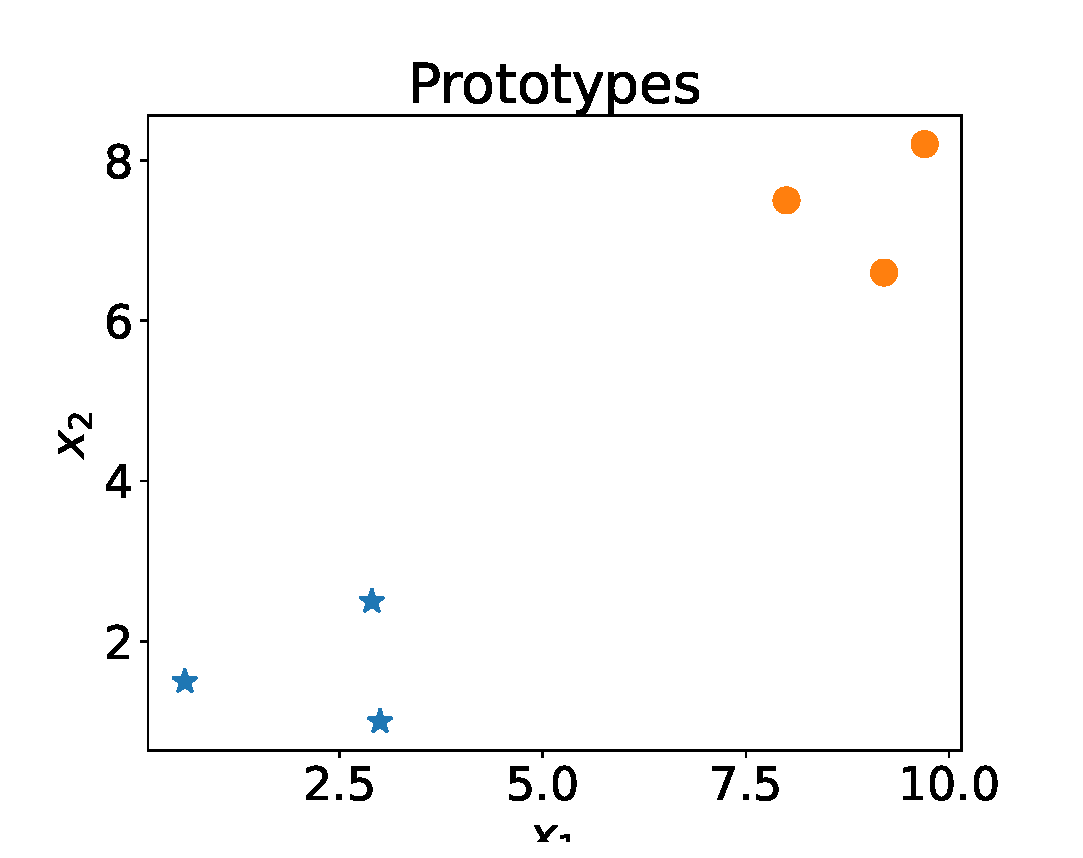
\includegraphics[width=.75\textwidth]{images/prototypes_0.eps}
  \caption{Prototypes of different categories}
  \label{fig:prototypes_0}
\end{figure}

We can also distinguish between two categories. For example, we could have a category of $\bigtriangleup$ and a category of $\bigcirc$.
Now, the question is: \textit{What do we do if we get a new data point?} For example $\vec{x}_{\times} = \begin{pmatrix}7.5\\4.0\end{pmatrix}$

\begin{figure}[h]
  \centering
  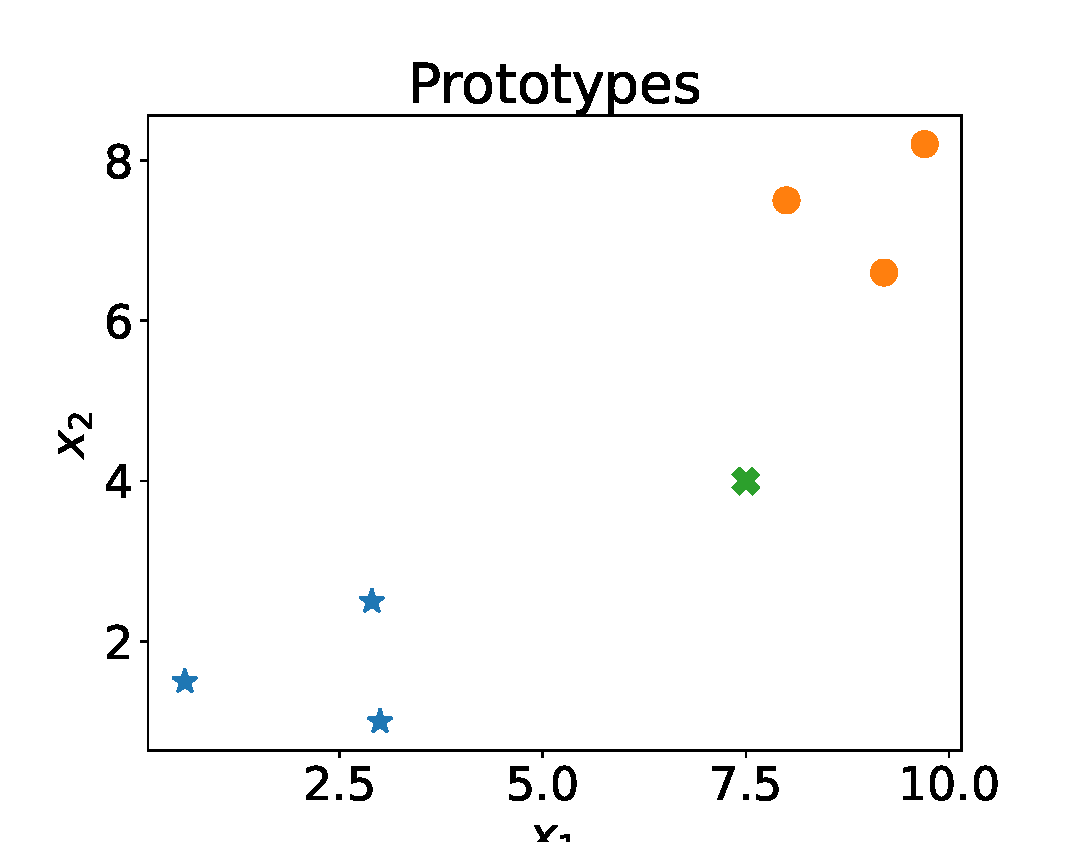
\includegraphics[width=.75\textwidth]{images/prototypes_1.eps}
  \caption{A new sample was added to the data set}
  \label{fig:prototypes_1}
\end{figure}

We need to find a mechanism of assigning a label to a new data point \textit{cross}.
For existing points we have this information already and we know which point belongs to which category. 
So how do we know which category the new point belongs to?

Psychiologists came up with the idea of designing so called \textit{prototypes} for each category.

This easiest solution for such prototype is calculating the \underline{mean} of all points in a category.
In this example we would compute the mean of all $\bigtriangleup$ $\vec{\mu}_\bigtriangleup$ and the mean of all $\bigcirc$ $\vec{\mu}_\bigcirc$.
\begin{figure}[h]
  \centering
  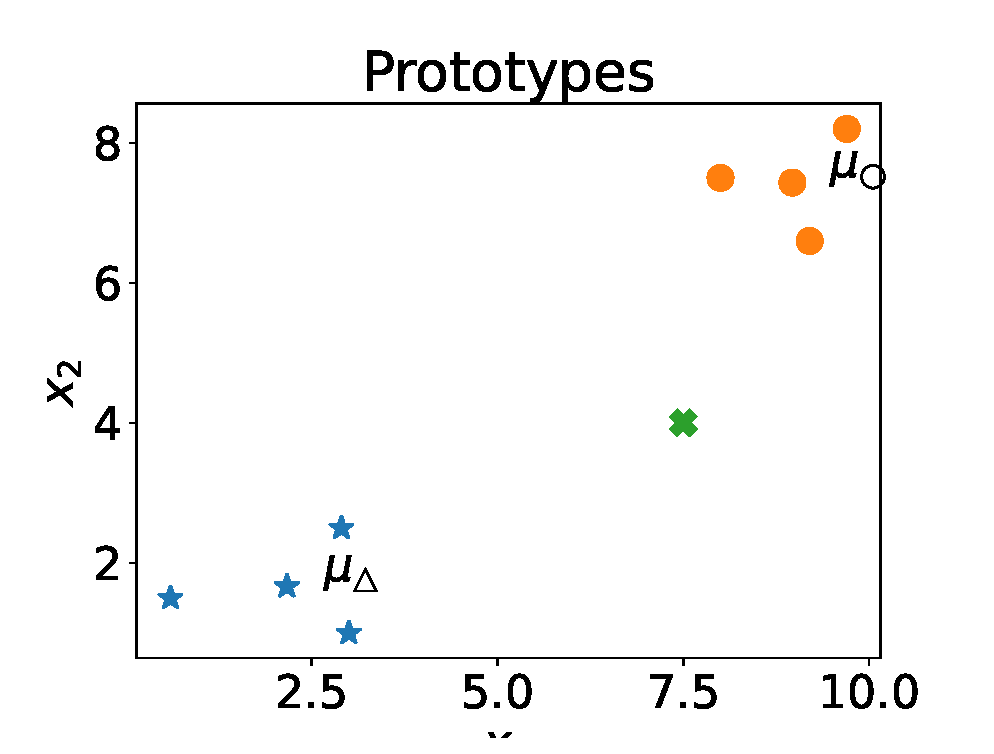
\includegraphics[width=.75\textwidth]{images/prototypes_2.eps}
  \caption{Mean values as prototypes for different categories are used to determine the label of a new data point}
  \label{fig:prototypes_2}
\end{figure}

The formula for the mean is:
\begin{equation}
  \vec{\mu} = \frac{1}{N} \sum_{i=1}^{N} x_i
  \label{eq:mean}
\end{equation}
where $N$ is the number of samples and $x_i$ is the $i$-th sample.
For each of the categories this translates to
\begin{align}
  \vec{\mu}_\bigtriangleup &= \frac{1}{N_\bigtriangleup} \sum_{i=1}^{N_\bigtriangleup} x_{\bigtriangleup, i} \\
  \vec{\mu}_\bigcirc &= \frac{1}{N_\bigcirc} \sum_{i=1}^{N_\bigcirc} x_{\bigcirc, i}
\end{align}
A label for a new data point $\vec{x}_{\times}$ can now be assigned by calculating the distance to each of the prototypes $\vec{\mu}_{\bigtriangleup}$ and $\vec{\mu}_{\bigcirc}$ and assigning the label of the prototype with the smallest distance.

One method to compute these distances is the \textbf{Euclidean Distance}, which is defined as
\begin{equation}
  d(\vec{x}, \vec{y}) = \sqrt{\sum_{i=1}^{N} (x_i - y_i)^2} = \sqrt{(\vec{x} - \vec{y})^T (\vec{x} - \vec{y})}
\end{equation}
where $n$ is the number of dimensions of the vectors $\vec{x}$ and $\vec{y}$.
There are many more distance metrics, and throughout this book we will encounter a few of them, but for now we will stick to the Euclidean Distance.
After computing all distances they can be compared and the label of the prototype with the smallest distance can be assigned to the new data point.
Mathematically this can be written as
\begin{equation}
  k^* = \argmin_{k\in\{1,\dots,K\}} d(\vec{x}, \vec{\mu}_k)
  \label{eq:nearest_centroid_inference}
\end{equation}
with $k^*$ being the label of the new data point $\vec{x}$ and $K$ being the number of categories.

\textbf{Congratulations!} You just implemented your first classification algorithm, the Nearest Centroid Classifier.
\section{Implementation}
In the following, we will look into different implementations of the NCC algorithm. And will look into two different approaches to compute the prototypes.
These two approaches can be used in most common Machine Learning algorithms.

\subsection{Inference}
The pseudo code to perform a classification (inference) using the NCC algirithm is very simple:
\begin{algorithm}
\LinesNumbered
\caption{\textbf{N}earest \textbf{C}entroid \textbf{C}lassifier Inference}\label{alg:ncc}
\KwData{$\vec{x}\in\mathbb{R}^D, \vec{\mu}_k, k\in\{1,\dots,K\}$}
\KwResult{$k^*$}
\Comment*[h]{Compute nearest class centroid}\\
$k^* \gets \argmin_{k\in\{1,\dots,K\}} d(\vec{x}, \vec{\mu}_k)$\;
\end{algorithm}

There are different ways to compute the centroids, here we used the means.
To compute the means we can use two different approaches, we call these approaches \textit{batch} and \textit{streaming}.
These terms might not 100\% match the common understanding of these terms, but we will use them to distinguish between the two approaches.

\textbf{Batched} refers to the fact that we compute the mean of all samples in a category at once. This approach requires
us to store all samples in memory and then compute the mean. This is the easier, but more expensive approach.

\textbf{Streaming} refers to the fact that we compute the mean of all samples in a category one by one. This approach does not require
us to store all samples in memory and is therefore more memory efficient. This approach is also called \textit{online} learning.

\subsection{Batched}
The batched approach is the easier one to implement. We simply store all samples in memory and then compute the mean.
\begin{algorithm}
\LinesNumbered
\caption{\textbf{NCC} Means (Batched)}\label{alg:ncc_batched}
\KwData{$\vec{x}\in\mathbb{R}^D, \vec{\mu}_k, k\in\{1,\dots,K\}$}
\KwResult{means $\vec{\mu}_k, k\in\{1\dots k\}$}
\Comment*[h]{Init means and counters for each class}\\
\Comment*[h]{Computation of class means}\\
\For{class $k$ in $K$}{
  $\vec{\mu}_k \gets \frac{1}{N_k}\sum^{N_k}_{i=1}\vec{x_i}$\;
}
\end{algorithm}

\subsection{Streaming}
To derive the streaming approach we need to look at the mathematical definition of the batched version
\begin{equation}
  \vec{\mu}_k = \frac{1}{N_k}\sum^{N_k}_{i=1}\vec{x_i}
\end{equation}
Imagine now, that we don't actually have the $N$-th data point yet.
We can rewrite the equation as
\begin{equation}
  \vec{\mu}_k = \frac{1}{N_k}\sum^{N_k-1}_{i=1}\vec{x_i} + \frac{1}{N_k}\vec{x_{N_k}}
\end{equation}
We can see the factor $\frac{1}{N_k}$ is the same for all terms. This factor can be rewritten a bit differently
\begin{equation}
  \frac{1}{N_k} = \frac{1}{N_k-1} \cdot \frac{N_k-1}{N_k}
\end{equation}
Now we can rewrite the equation as
\begin{equation}
  \vec{\mu}_k = \frac{1}{N_k}\sum^{N_k-1}_{i=1}\vec{x_i} + \frac{1}{N_k} \cdot \vec{x_{N_k}} = \frac{N_k - 1}{N_k}\frac{1}{N_k-1}\sum^{N_k-1}_{i=1}\vec{x_i} + \frac{1}{N_k} \cdot \vec{x_{N_k}}
\end{equation}
If we compare the middle term $\frac{1}{N_k}\sum^{N_k-1}_{i=1}\vec{x_i}$ with the original equation \eqref{eq:mean} we can see that it is just the mean of the previous iteration $\vec{\mu}_{k-1}$
\begin{equation}
  \Rightarrow \vec{\mu}_{k} = \frac{N_k - 1}{N_k}\vec{\mu}_{k-1} + \frac{1}{N_k} \cdot \vec{x_k}
  \label{eq:iterative-mean}
\end{equation}

This equation can be used to iteratively compute the mean of a category. We can start with $\vec{\mu}_0 = \vec{0}$ and then compute the mean of each sample by using the equation \eqref{eq:iterative-mean}.
An implementation of this approach is shown in Algorithm \ref{alg:ncc_streaming}.
\begin{algorithm}
\LinesNumbered
\caption{\textbf{NCC} Means (Streaming)}\label{alg:ncc_streaming}
\KwData{$\vec{x}\in\mathbb{R}^D$ labels $y_1, \dots, y_N\in\{1,\dots,K\}$}
\KwResult{means $\vec{\mu}_k, k\in\{1\dots k\}$}
\Comment*[h]{Init means and counters for each class}\\
$\forall k:$ $\vec{\mu}_k \gets \vec{0}, N_k = 0$\;
\For{Data point $i = 1,\dots,N$}{
  \Comment*[h]{Update means and counters}\\
  $k \gets y_i$\;
  $\vec{\mu}_k \gets \frac{N_k}{N_k + 1}\vec{\mu}_{k} + \frac{1}{N_k + 1} \cdot \vec{x_i}$\;
  $N_k \gets N_k + 1$\;
}
\end{algorithm}
As you can see for this iterative approach we only need to store all $\vec{\mu}_k$ and $N_k$ in memory. This is a huge advantage over the batched approach, especially if we have a lot of data.

You can see a visualization of the two approaches in Figure \ref{fig:ncc_batched_streaming}.

\section{Limitations}
Once we implemented one of the two approaches we can use it to classify new data points. For the example above this might result in \textit{Decision Boundaries} as shown in Figure \ref{fig:ncc_db_uncorrelated}.
This brings up a new group of questions, specifically about the limitations of the NCC or when 
should we use the NCC and when should we not use it.


The NCC is a very simple algorithm and therefore has some limitations.
\begin{enumerate}
  \item NCC should only be used for uncorrelated data, i.e. $x_1$ and $x_2$ are independent/without any correlation.
    The background here is the prediction by the model, the line between the two colors in Figure \ref{fig:ncc_db_uncorrelated} is called the \textit{Decision Boundary} (DB). We see that
    we have not a single miss-classification in this example. But this doesn't apply to all cases.
    Occasionally we will witness miss-classifications even in simple examples.
    This is due to the fact that the NCC is a linear classifier and therefore can only separate linearly separable data. Whenever we have \textit{outliers}, \textit{mislabeled data} or \textit{noise} in the input data, it is inevidable that the NCC will not be able to separate the data with full accuracy.
  \item The NCC does not consider correlation when classifying. It only computes and copares mean values of the data.\\
    Compare the decision boundaries in Figure \ref{fig:ncc_db_uncorrelated} and Figure \ref{fig:ncc_db_correlated}. In Figure \ref{fig:ncc_db_correlated} we see that the decision boundary is not optimal, several data points of the blue class would be classified as orange and vice versa.
    If we compute only the means, we can not successfully separate the correlated data with a single DB.
  \item This also applies to a problem with more than two classes. If we have more than two classes, we can not use a single DB to separate the data.
    We would need to compute multiple DBs to separate the data, as visualized in Figure \ref{fig:ncc_db_3_class}.
\end{enumerate}

\begin{figure}[h]
  \centering
  \begin{minipage}{.45\textwidth}
  \centering
    \includesvg[width=.95\textwidth]{images/NCC_uncorrelated.svg}
    \caption{Decision Boundaries for uncorrelated data}
    \label{fig:ncc_db_uncorrelated}
  \end{minipage}
  \hfill
  \begin{minipage}{.45\textwidth}
  \centering
    \includesvg[width=.95\textwidth]{images/NCC_correlated.svg}
    \caption{Decision Boundaries for correlated data}
    \label{fig:ncc_db_correlated}
  \end{minipage}\newline
  \hfill
  \begin{minipage}{.45\textwidth}
  \centering
    \includesvg[width=.95\textwidth]{images/NCC_3_class.svg}
    \caption{Decision Boundaries for 3 classes}
    \label{fig:ncc_db_3_class}
  \end{minipage}
  \hfill
\end{figure}

\section{Linear Classification}
In the previous section we motivated the NCC by using a psychological model. We also saw that the NCC is good for uncorrelated data, data that is linear separable.\\
Under the hood the NCC is computing Decision Boundaries to separate the data, this DB is a line in the feature space.
This puts the NCC algorithm into the group of \textit{Linear Classifiers}. Linear Classifiers are a group of algorithms that perform well on linearly separable data, just like the NCC.
The NCC is a very simple linear classifier, but there are more complex ones. We will look into some of them in later chapters.
But what is this line that separates the data? How can we compute it?\\
We will look into this now in a more mathematical way.
\subsection{From Prototypes to Linear Classification}
Now we will use the definition of NCC \eqref{eq:nearest_centroid_inference} to derive general linear classification.
Let $\vec{x} \in \mathbb{R}^D$ be a data point and $\vec{\mu}_k \in \mathbb{R}^D$ be the prototype of class $k$. For two classes this would be $\vec{\mu}_0$ and $\vec{\mu}_1$.

Then we would find the class of $\vec{x}$ by computing the distance to each prototype and assigning the label of the prototype with the smallest distance.
\begin{equation}
  k^* = \argmin_{k\in\{1,\dots,K\}} d(\vec{x}, \vec{\mu}_k)
\end{equation}
or
\begin{align}
  k^* &= \argmin(d(\vec{x}, \vec{\mu}_0), d(\vec{x}, \vec{\mu}_1))\\
  \Leftrightarrow&\, d(\vec{x}, \vec{\mu}_0) > d(\vec{x}, \vec{\mu}_1)
\end{align}
This is the same as saying that $\vec{x}$ is closer to $\vec{\mu}_0$ than to $\vec{\mu}_1$. We can write this as
\begin{align}
  \Leftrightarrow& \norm{\vec{x} - \vec{\mu}_0}_2^2 > \norm{\vec{x} - \vec{\mu}_1}_2^2
\end{align}
where $\norm{\cdot}_2$ is the Euclidean norm. We can square both sides of the inequality and get
\begin{align}
  \Rightarrow& \norm{\vec{x} - \vec{\mu}_0}_2 > \norm{\vec{x} - \vec{\mu}_1}_2
\end{align}
We can now expand the Euclidean norm to get
\begin{align}
  \Rightarrow\, & \vec{x}^T\vec{x} - 2\vec{x}^T\vec{\mu}_0 + \vec{\mu}_0^T\vec{\mu}_0 > \vec{x}^T\vec{x} - 2\vec{x}^T\vec{\mu}_1 + \vec{\mu}_1^T\vec{\mu}_1 \\
  \Leftrightarrow\, & - 2\vec{x}^T\vec{\mu}_0 + \vec{\mu}_0^T\vec{\mu}_0 > - 2\vec{x}^T\vec{\mu}_1 + \vec{\mu}_1^T\vec{\mu}_1 \\
  \Leftrightarrow\, & \vec{\mu}_0^T\vec{x} - \frac{\vec{\mu}_0^T\vec{\mu}_0}{2} < \vec{\mu}_1^T\vec{x} - \frac{\vec{\mu}_1^T\vec{\mu}_1}{2} \\
  \Leftrightarrow\, & 0 < (\underbrace{\vec{\mu}_0-\vec{\mu}_1}_{\vec{\omega}})^T\vec{x} - \underbrace{\frac{1}{2}\left(\vec{\mu}_0^T\vec{\mu}_0-\vec{\mu}_1^T\vec{\mu}_1\right)}_{\beta}
\end{align}
$\vec{\omega}$ is called the \textit{weight vector}, for NCC this is the difference vector between both means.
$(\vec{\mu}_0-\vec{\mu}_1)^T\vec{x}$ is called the \textit{activation} of the input $\vec{x}$. From the previous chapter \ref{ch:math} we know that this is essentially just projecting $\vec{x}$ onto the difference vector, which will result in a constant value.
The constant value is then compared to the bias $\beta$ and if it is greater than $\beta$ the input is classified as class $0$, otherwise as class $1$.
In other words
\begin{equation}
  0 < \vec{\omega}^T\vec{x} + \beta
  \label{eq:linear_classifier}
\end{equation}
This is the general form of a linear classifier.
Using this general form we can now compute the DB for the NCC example

\begin{minipage}{.45\textwidth}
  {
  \centering
\begin{align}
  \vec{\tilde{x}} &= \left(\vec{{\omega}}^T\vec{x}\right) \\
  \vec{\tilde{x}} - \beta &= \left\{\begin{matrix}
    > 0 & \text{class } 0 \\
    < 0 & \text{class } 1
  \end{matrix}\right.
\end{align}
  }
with class $0$ the orange class and class $1$ the blue class.
\end{minipage}
\begin{minipage}{.45\textwidth}
  \centering
  \includesvg[width=.95\textwidth]{images/NCC_lin_classifier.svg}
  \caption{NCC as linear classifier, the blue line visualizes the decision boundary $\vec{\omega}$ and the green line is the decision threshold $\beta$}
  \label{fig:ncc_linear_classifier}
\end{minipage}
\vspace{1cm}

This is more or less all we need to know from linear classifiers and we can now derive it from the NCC algorithm.

\subsection{Linear Classification}
We will now look a bit deeper into linear classification.
Linear classification algorithms predict classes for given data points $\vec{x}$ by computing the activation of the input $\vec{x}$ and comparing it to a bias $\beta$
\begin{equation}
  f(\vec{x}) = \vec{\omega}^T\vec{x} + \beta
  \label{eq:linear_classification}
\end{equation}
where $\vec{\omega}$ is the decision boundary and $\beta$ is the decision threshold.
For two classes $\vec{\omega}$, the difference of the class means, is a vector and $\beta$ is a scalar
\begin{equation}
  \vec{\omega}_{\text{NCC}} = \vec{\mu}_0 - \vec{\mu}_1
\end{equation}
There are other ways to calculate $\vec{\omega}$ for other linear classifiers.
Using this definition we can build the NCC as a linear classification model
\begin{equation}
  f(\vec{x}) = \vec{\omega}_{\text{NCC}}^T\vec{x} + \beta_{\text{NCC}}
\end{equation}

What does this geometrically mean?\\
First, we assume our data is sepearable by the diagonal through the 2nd and 4th quadrant. This is the same as saying that the data is linearly separable and we won't need a threshold $\beta$ for now.
$\vec{\omega}$ is parallel to ${\vec{\mu}_0-\vec{\mu}_1}$ and therefore orthogonal to the DB.
Then any point above the DB, perpendicular to $\vec{\omega}$, will be classified as class $0$ and any point below the DB will be classified as class $1$. You can see a visualization of that in Figure \ref{fig:linear_classifier_origin}.

\begin{minipage}{.45\textwidth}
  \centering
  \includesvg[width=.95\textwidth]{images/linear_classifier_origin.svg}
  \caption{Linear Classifier without bias}
  \label{fig:linear_classifier_origin}
\end{minipage}
\hfill
\begin{minipage}{.45\textwidth}
  \centering
  \includesvg[width=.75\textwidth]{images/linear_classifier_origin_bias.svg}
  \caption{Linear Classifier with bias}
  \label{fig:linear_classifier_origin_bias}
\end{minipage}

Now, let's look at the bias value $\beta$. Figure \ref{fig:linear_classifier_origin_bias} demonstrates that the bias is the value that is added to the activation of the input $\vec{x}$.
You can literally say that we simply shift our DB up or down along the $x_2$-axis by $\beta$.


\framedtext{\color{red}{TODO:} Add more details about linear classification, add linear classifier plots}

